\clearpage
\VerdierPhysicalPageAnchor{0082}%
\VerdierSemanticAnchor{ch1-3}
\section{Triangles distingués}

\VerdierSemanticAnchor{ch1-3-1}
\subsection{Le cône d'un morphisme}

\VerdierSemanticAnchor{ch1-3-1-1}
\noindent\textbf{3.1.1.}\quad
\VerdierSemanticAnchor{ch1-3-1-1-tr1-category}
Soit $C$ une catégorie additive. On désigne par
$\operatorname{tr}_1(C)$ la catégorie suivante :

\VerdierSemanticAnchor{ch1-3-1-1-objects}
\noindent--\quad Les objets de $\operatorname{tr}_1(C)$ sont les morphismes
(de degré zéro) $X\xrightarrow{f}Y$ de complexes d'objets de $C$.

\VerdierSemanticAnchor{ch1-3-1-1-morphisms}
\noindent--\quad Soient $X\xrightarrow{f}Y$ et
$X'\xrightarrow{f'}Y'$ deux objets de $\operatorname{tr}_1(C)$. Un morphisme
de $X\xrightarrow{f}Y$ dans $X'\xrightarrow{f'}Y'$ est un triplet
$(g,h,a)$, où $g\colon X\longrightarrow X'$ et
$h\colon Y\longrightarrow Y'$ sont des morphismes de complexes de degré zéro
et où
\VerdierSemanticAnchor{ch1-3-1-1-homotopy-data}
$a\colon f'g\rightsquigarrow hf$ est une homotopie reliant $f'g$ à $hf$.

\VerdierSemanticAnchor{ch1-3-1-1-composition}
\noindent--\quad Soient
\begin{equation*}
  \begin{aligned}
    (g,h,a)\colon (X\xrightarrow{f}Y)
      &\longrightarrow (X'\xrightarrow{f'}Y'),\\
    (g',h',a')\colon (X'\xrightarrow{f'}Y')
      &\longrightarrow (X''\xrightarrow{f''}Y'')
  \end{aligned}
\end{equation*}
deux morphismes de $\operatorname{tr}_1(C)$. Le morphisme composé
\begin{equation*}
  (g'',h'',a'')\colon
  (X\xrightarrow{f}Y)\longrightarrow(X''\xrightarrow{f''}Y'')
\end{equation*}
est alors défini par les égalités :

\VerdierSemanticAnchor{ch1-3-1-1-eq1}
\begin{equation}
  \begin{aligned}
    g''&=g'g,\\
    h''&=h'h,\\
    a''&=a'\star g+h'\star a.
  \end{aligned}
  \tag{3.1.1.1}
\end{equation}

\VerdierSemanticAnchor{ch1-3-1-1-category-verification}
On vérifie aussitôt qu'on a bien ainsi défini une catégorie.
\VerdierSemanticAnchor{ch1-3-1-1-diagram-representation}
On représentera le plus souvent un morphisme
$(g,h,a)\colon(X\xrightarrow{f}Y)\longrightarrow
(X'\xrightarrow{f'}Y')$ de $\operatorname{tr}_1(C)$ par un diagramme :

\VerdierSemanticAnchor{ch1-3-1-1-eq2}
\begin{equation}
  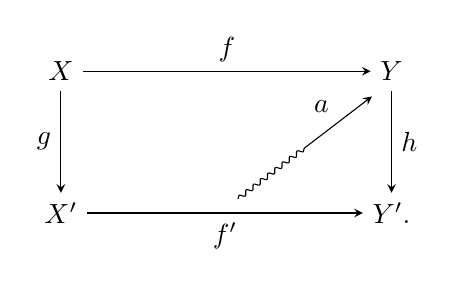
\begin{tikzpicture}[>=stealth,baseline=(current bounding box.center)]
    \node (X)  at (0,1.8) {$X$};
    \node (Y)  at (4.2,1.8) {$Y$};
    \node (Xp) at (0,0) {$X'$};
    \node (Yp) at (4.2,0) {$Y'\mathpunct{.}$};
    \draw[->] (X) -- node[above] {$f$} (Y);
    \draw[->] (X) -- node[left] {$g$} (Xp);
    \draw[->] (Y) -- node[right] {$h$} (Yp);
    \draw[->] (Xp) -- node[below] {$f'$} (Yp);
    \draw[decorate,decoration={snake,amplitude=0.8pt,segment length=3.3pt}]
      (2.25,0.18) -- (3.10,0.83);
    \draw[->] (3.10,0.83) -- node[above left] {$a$} (3.95,1.48);
  \end{tikzpicture}
  \tag{3.1.1.2}
\end{equation}
